% why13.tex — Why 13? The Fano plane, the split Cayley hexagon, and the
% Meinhold-72 Hecke algebra H(G2(2), PSL(3,2)).
%
% Expository paper (pedagogical, for ourselves). Companion computations:
%   why13_fano.g, why13_orbitals.g (GAP), outputs in why13_orbitals.out.
% Authoritative algebra tables: MEINHOLD-HECKE.md, meinhold_hecke.g.
%
% Build: pdflatex why13.tex (twice)

\documentclass[11pt]{article}
\usepackage[margin=2.7cm]{geometry}
\usepackage{amsmath,amssymb,amsthm,mathtools}
\usepackage{booktabs}
\usepackage{tikz}
\usetikzlibrary{calc,positioning}
\usepackage[colorlinks=true,linkcolor=blue!50!black,citecolor=blue!50!black]{hyperref}

\newtheorem{theorem}{Theorem}[section]
\newtheorem{lemma}[theorem]{Lemma}
\newtheorem{proposition}[theorem]{Proposition}
\newtheorem{corollary}[theorem]{Corollary}
\theoremstyle{definition}
\newtheorem{definition}[theorem]{Definition}
\newtheorem{example}[theorem]{Example}
\newtheorem{nonexample}[theorem]{Non-example}
\newtheorem{remark}[theorem]{Remark}
\newtheorem{question}[theorem]{Question}
\newtheorem{fact}[theorem]{Fact}

\newcommand{\F}{\mathbb{F}}
\newcommand{\C}{\mathbb{C}}
\newcommand{\Z}{\mathbb{Z}}
\newcommand{\PG}{\mathrm{PG}}
\newcommand{\GH}{\mathrm{GH}}
\newcommand{\PSL}{\mathrm{PSL}}
\newcommand{\PSU}{\mathrm{PSU}}
\newcommand{\GL}{\mathrm{GL}}
\newcommand{\Aut}{\mathrm{Aut}}
\newcommand{\Sym}{\mathrm{Sym}}

\title{Why 13?\\[2mm]\large The Fano plane, the split Cayley hexagon $\GH(2,2)$,\\
and the Hecke algebra $H(G_2(2),\PSL(3,2))$}
\author{Fable (Claude), with Robin Langer}
\date{June 2026 --- a living document}

\begin{document}
\maketitle

\begin{abstract}
The Hecke algebra $H(G_2(2),\PSL(3,2))$ --- discovered in the ``Meinhold-72''
sessions --- has a two-dimensional irreducible representation generated by two
matrices $A,B$ with
\[
A^2 = I,\qquad B^2 = 13\,I,\qquad AB+BA = -4I .
\]
Where does the $13$ come from? This paper explains \emph{everything} needed to
answer that: what a Fano plane is (six definitions), what the split Cayley
hexagon is (four definitions), how they are related (Fano planes are
generalized triangles, hexagons are generalized hexagons; $\PSL(3,2)$ sits
inside $G_2(2)$ in exactly $72$ ways, each fixing a chiral Fano structure), and
finally a complete combinatorial derivation of
\[
13 \;=\; 7 + 2\cdot 3,
\]
where $7$ is an orbital valency and $3 = \sqrt{k-\mu}$ is an eigenvalue of the
strongly regular graph $\mathrm{SRG}(36,21,12,12)$ on the $36$ Fano structures
of one chirality. All computational claims are verified in GAP
(\texttt{why13\_fano.g}, \texttt{why13\_orbitals.g}).
\end{abstract}

\tableofcontents

%======================================================================
\section{Introduction: the question}
%======================================================================

The group $G = G_2(2)$ of order $12096 = 2^6\cdot 3^3\cdot 7$ acts primitively
on $63$ points (\texttt{PrimitiveGroup(63,2)} in GAP). It contains a subgroup
$K \cong \PSL(3,2)$ of order $168$ and index $72$, unique up to conjugacy. The
double cosets $K\backslash G/K$ give a Hecke algebra
\[
H(G,K) \;\cong\; \C \oplus \C \oplus M_2(\C) \oplus \C \oplus \C
\]
of rank $8$, with canonical basis $T_1,\dots,T_8$ of valencies
$1,1,7,7,7,7,21,21$. In the $2$-dimensional Wedderburn block, the images
$A = \rho(T_2)$ and $B = \rho(T_3)$ satisfy
\[
A^2 = I, \qquad B^2 = 13\,I, \qquad AB + BA = -4I.
\]
The relation $B^2 = 13I$ is forced by the structure constants: in the algebra,
\begin{equation}\label{eq:T3sq}
T_3 \cdot T_3 \;=\; 7\,T_1 + 2\,T_8,
\end{equation}
and $T_8$ is \emph{central} with $\rho(T_8) = 3I$, so
$B^2 = 7I + 2\cdot 3I = 13I$. The question ``why 13?'' therefore splits into:
\begin{enumerate}
\item Why does $T_3^2$ hit only the identity and the central element $T_8$,
with coefficients $7$ and $2$? (Combinatorics of the orbital graphs.)
\item Why does the central element act by the scalar $3$? (Spectral theory of a
strongly regular graph.)
\end{enumerate}
Both questions are about the geometry of \emph{Fano planes living inside the
split Cayley hexagon}. So we start from scratch.

%======================================================================
\section{Incidence geometry and the Fano plane}
%======================================================================

\subsection{Incidence structures and projective planes}

\begin{definition}[Incidence structure]
An \emph{incidence structure} is a triple $(\mathcal P, \mathcal L, \mathrm I)$
where $\mathcal P$ is a set of \emph{points}, $\mathcal L$ a set of
\emph{lines}, and $\mathrm I \subseteq \mathcal P \times \mathcal L$ an
\emph{incidence relation}. We write $p \in \ell$ for $(p,\ell)\in\mathrm I$
when lines are identified with their point sets. A \emph{flag} is an incident
pair $(p,\ell)$; an \emph{antiflag} is a non-incident pair.
\end{definition}

\begin{definition}[Projective plane]\label{def:projplane}
A \emph{projective plane} is an incidence structure such that:
\begin{enumerate}
\item[(P1)] any two distinct points lie on exactly one common line;
\item[(P2)] any two distinct lines meet in exactly one common point;
\item[(P3)] (non-degeneracy) there exist four points, no three collinear.
\end{enumerate}
A plane has \emph{order} $n$ if some (equivalently every) line has $n+1$
points; then every point is on $n+1$ lines, and there are $n^2+n+1$ points and
$n^2+n+1$ lines.
\end{definition}

\begin{example}
The real projective plane $\mathbb{RP}^2$ satisfies (P1)--(P3) but is infinite.
The smallest possible order is $n = 2$: lines of $3$ points, $7$ points,
$7$ lines.
\end{example}

\begin{nonexample}
The \emph{near-pencil}: points $\{1,2,3,4\}$, lines
$\{1,2,3\},\{1,4\},\{2,4\},\{3,4\}$. It satisfies (P1) and (P2) but fails (P3):
every set of four points contains three on the line $\{1,2,3\}$ or includes
point $4$ twice. Degenerate ``planes'' like this are exactly what (P3)
excludes.
\end{nonexample}

\subsection{The Fano plane: six definitions}

\begin{definition}[Fano plane, axiomatic]\label{def:fano-ax}
The \emph{Fano plane} is the (unique, by
Theorem~\ref{thm:fano-unique}) projective plane of order $2$: $7$ points, $7$
lines, $3$ points per line, $3$ lines per point.
\end{definition}

\begin{figure}[ht]
\centering
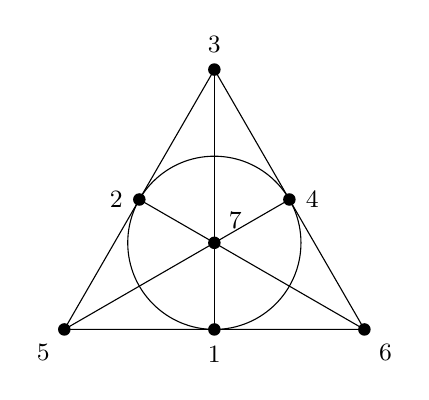
\begin{tikzpicture}[scale=2.2,
  pt/.style={circle,fill=black,inner sep=1.6pt},
  lab/.style={font=\small}]
  % corners 3 (top), 5 (bottom left), 6 (bottom right); center 7
  \coordinate (A) at (90:1);    % 3
  \coordinate (B) at (210:1);   % 5
  \coordinate (C) at (330:1);   % 6
  \coordinate (O) at (0,0);     % 7
  \coordinate (Mab) at ($(A)!0.5!(B)$); % 2 on side 3-5
  \coordinate (Mac) at ($(A)!0.5!(C)$); % 4 on side 3-6
  \coordinate (Mbc) at ($(B)!0.5!(C)$); % 1 on side 5-6
  % sides
  \draw (A) -- (B) -- (C) -- cycle;
  % medians
  \draw (A) -- (Mbc); \draw (B) -- (Mac); \draw (C) -- (Mab);
  % circle line {1,2,4}
  \draw (O) circle ({0.5});
  \node[pt,label={[lab]above:$3$}]  at (A) {};
  \node[pt,label={[lab]below left:$5$}]  at (B) {};
  \node[pt,label={[lab]below right:$6$}] at (C) {};
  \node[pt,label={[lab]above right:$7$}] at (O) {};
  \node[pt,label={[lab]left:$2$}]  at (Mab) {};
  \node[pt,label={[lab]right:$4$}] at (Mac) {};
  \node[pt,label={[lab]below:$1$}] at (Mbc) {};
\end{tikzpicture}
\caption{The Fano plane with the difference-set labelling
$\ell_i = \{i+1,\,i+2,\,i+4\} \pmod 7$. The seven lines are the three sides
$\{5,6,1\},\{2,3,5\},\{3,4,6\}$, the three medians
$\{7,1,3\},\{4,5,7\},\{6,7,2\}$, and the circle $\{1,2,4\}$. Check: each is a
translate of $\{1,2,4\}$ mod $7$.}
\label{fig:fano}
\end{figure}

\begin{definition}[Fano plane as $\PG(2,2)$]\label{def:fano-pg}
Let $V = \F_2^3$. Points are the $7$ one-dimensional subspaces
($=$ nonzero vectors, since $|\F_2^\times| = 1$); lines are the $7$
two-dimensional subspaces ($=$ kernels of nonzero linear functionals). A point
lies on a line iff the vector lies in the subspace. Equivalently: three nonzero
vectors $u,v,w$ are collinear iff $u + v + w = 0$.
\end{definition}

\begin{example}
Write each point $i\in\{1,\dots,7\}$ in binary: $1=001$, $2=010$, $3=011$,
$4=100$, $5=101$, $6=110$, $7=111$. Then $\{1,2,3\}$ is a line since
$001\oplus010\oplus011 = 000$. (This binary labelling is the Hamming-code
labelling; it differs from the difference-set labelling of
Figure~\ref{fig:fano} by a relabelling.)
\end{example}

\begin{definition}[Fano plane as a Steiner system]\label{def:fano-steiner}
A \emph{Steiner system} $S(2,3,7)$ is a collection of $3$-element blocks of a
$7$-set such that every $2$-subset lies in exactly one block. Any $S(2,3,7)$
is a Fano plane: axiom (P1) is the Steiner condition, and (P2) follows by
counting --- two blocks meeting in $\geq 2$ points would violate uniqueness,
and two disjoint blocks would leave the pairs across them uncovered by a
count: each block covers $3$ pairs, $7$ blocks cover $21 = \binom72$ pairs
exactly once, and through a point $p$ outside a block $\ell$ the three lines
$p q$ ($q\in\ell$) are distinct, so they exhaust the $3$ lines through $p$;
hence no line through $p$ misses $\ell$.
\end{definition}

\begin{definition}[Fano plane from a perfect difference set]\label{def:fano-diff}
$D = \{1,2,4\} \subset \Z/7$ is a \emph{perfect difference set}: every nonzero
residue mod $7$ arises exactly once as a difference $d - d'$ with $d,d'\in D$.
(Check: $2{-}1{=}1$, $4{-}2{=}2$, $4{-}1{=}3$, $1{-}4{=}4$, $2{-}4{=}5$,
$1{-}2{=}6$.) The translates $\ell_i = i + D$ ($i \in \Z/7$) are the lines of a
Fano plane on the points $\Z/7$: the pair $\{x,y\}$ lies on $\ell_i$ iff
$x-i, y-i \in D$, and since $x - y$ has a \emph{unique} representation as a
difference of elements of $D$, there is exactly one such $i$.
\end{definition}

\begin{nonexample}
$D' = \{0,1,2\}$ is \emph{not} a perfect difference set: its differences are
$\pm1, \pm2$ only, so $3$ and $4$ never occur. Concretely, the translates of
$D'$ give $7$ triples in which the pair $\{0,3\}$ lies on \emph{no} line ---
axiom (P1) fails. ``Seven triples covering each point three times'' is not
enough; the difference structure is essential.
\end{nonexample}

\begin{definition}[Fano plane as octonion multiplication mnemonic]\label{def:fano-oct}
Label the seven imaginary units of the octonions $e_1,\dots,e_7$ and decree
$e_i e_{i+1} = e_{i+3}$ (indices mod $7$), extended by the rules
$e_i^2 = -1$ and anticommutativity. The triples $\{i, i{+}1, i{+}3\}$ are the
lines of a Fano plane (the difference set $\{0,1,3\}$ works just like
$\{1,2,4\}$: its differences $1,3,2,6,4,5$ cover everything once). Each
oriented line is a copy of the quaternions. The Fano plane with oriented lines
\emph{is} the multiplication table of the octonions.
\end{definition}

\begin{definition}[Fano plane via the Heawood graph]\label{def:fano-heawood}
The \emph{incidence graph} (Levi graph) of an incidence structure is the
bipartite graph on $\mathcal P \sqcup \mathcal L$ with edges the flags. The
Fano plane is the incidence structure whose incidence graph is the
\emph{Heawood graph}: the unique bipartite cubic graph of girth $6$ on $14$
vertices (Figure~\ref{fig:heawood}). In the language of
Section~\ref{sec:genpoly}: the Fano plane is the unique \emph{generalized
triangle of order $(2,2)$}. This is the definition that puts it in the same
family as the split Cayley hexagon.
\end{definition}

\begin{figure}[ht]
\centering
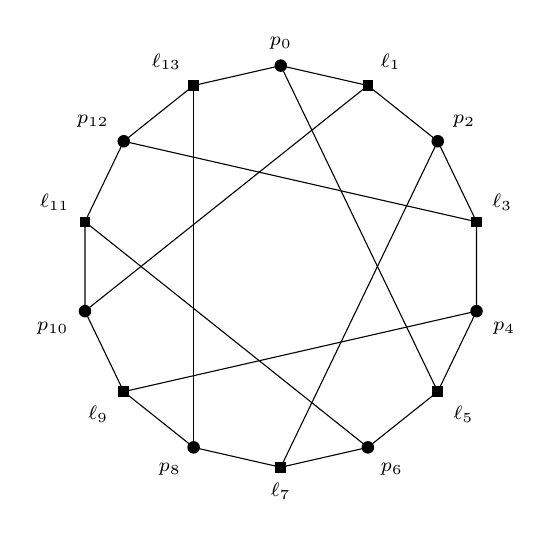
\begin{tikzpicture}[scale=1.7]
  \foreach \i in {0,...,13} {
    \coordinate (v\i) at ({90 - \i*360/14}:1.5);
  }
  \foreach \i [evaluate=\i as \j using {int(mod(\i+1,14))}] in {0,...,13} {
    \draw (v\i) -- (v\j);
  }
  \foreach \a/\b in {0/5, 2/7, 4/9, 6/11, 8/13, 10/1, 12/3} {
    \draw (v\a) -- (v\b);
  }
  \foreach \i in {0,2,4,6,8,10,12} {
    \node[circle,fill=black,inner sep=1.6pt,
      label={[font=\scriptsize]{90-\i*360/14}:$p_{\i}$}] at (v\i) {};
  }
  \foreach \i in {1,3,5,7,9,11,13} {
    \node[rectangle,fill=black,inner sep=1.9pt,
      label={[font=\scriptsize]{90-\i*360/14}:$\ell_{\i}$}] at (v\i) {};
  }
\end{tikzpicture}
\caption{The Heawood graph: a $14$-cycle plus the chords
$\{0,5\},\{2,7\},\{4,9\},\{6,11\},\{8,13\},\{10,1\},\{12,3\}$. Circles are
points, squares are lines of the Fano plane; girth $6$ encodes
``no digons'': two points on two common lines would give a $4$-cycle.}
\label{fig:heawood}
\end{figure}

\begin{theorem}[Uniqueness]\label{thm:fano-unique}
All projective planes of order $2$ are isomorphic.
\end{theorem}

\begin{proof}
Let $\Pi$ be a plane of order $2$; fix a line $\ell = \{a,b,c\}$ and a point
$d \notin \ell$ (exists by (P3)). The lines $da, db, dc$ are distinct and
account for all $3$ lines through $d$; each has one more point, giving points
$e \in da$, $f \in db$, $g \in dc$, and these are distinct (two of them equal
would put two lines through the pair $\{d,\cdot\}$). So
$\Pi = \{a,\dots,g\}$, $7$ points, and the incidences listed so far are
forced. The remaining $3$ lines each must join $e,f,g$ to the points of
$\ell$ not already joined to them; one checks there is exactly one way to
complete: e.g.\ the line through $e$ and $b$ cannot contain $a$ (that's
$\ell\,$? no --- $a,b \in \ell$, and $e\notin\ell$, so the line $eb \ne \ell$
and meets $\ell$ only in $b$), cannot contain $d$ or $f$ (lines $da$, $db$
already pass through those pairs), so its third point is forced to be $g$ or
$c$; and $ec$ would leave the pair $\{e,g\}$ uncoverable. Following these
forced choices yields a unique incidence table, so any two order-$2$ planes
admit an isomorphism mapping the chosen configurations to each other.
\end{proof}

\begin{fact}[Automorphisms]\label{fact:fano-aut}
$\Aut(\text{Fano}) \cong \GL(3,2) = \PSL(3,2) \cong \PSL(2,7)$, the simple
group of order $168 = 7\cdot 6\cdot 4$. From Definition~\ref{def:fano-pg},
any linear automorphism of $\F_2^3$ permutes the points and lines; the order
is $(2^3-1)(2^3-2)(2^3-2^2) = 7\cdot6\cdot4$. Conversely every plane
automorphism is induced by a linear map because a plane automorphism is
determined by its action on a quadrilateral (the proof of
Theorem~\ref{thm:fano-unique} shows a quadrilateral determines everything)
and $\GL(3,2)$ is transitive on quadrilaterals. The action on flags
($21$ of them) is transitive, as is the action on antiflags ($42 = 7\cdot 6$
of them). \emph{Remember these numbers: $21$ and $42$.}
\end{fact}

%======================================================================
\section{Generalized polygons}\label{sec:genpoly}
%======================================================================

\subsection{Definition and first examples}

\begin{definition}[Generalized $n$-gon]\label{def:genpoly}
A \emph{generalized $n$-gon} is an incidence structure whose incidence graph
$\Gamma$ (bipartite, on points $\sqcup$ lines) satisfies:
\begin{enumerate}
\item[(G1)] $\mathrm{diam}(\Gamma) = n$;
\item[(G2)] $\mathrm{girth}(\Gamma) = 2n$;
\item[(G3)] (thickness) every vertex has degree $\geq 3$.
\end{enumerate}
It has \emph{order} $(s,t)$ if every line has $s+1$ points and every point is
on $t+1$ lines. (Regularity is automatic from (G1)--(G3) for $n\geq 3$; we
take it as given.)
\end{definition}

The girth condition says: no ``short circuits.'' A cycle of length $2k < 2n$
in the incidence graph is a closed configuration of $k$ points and $k$ lines
--- an ordinary $k$-gon. So a generalized $n$-gon contains no ordinary
$k$-gons for $k < n$, while diameter $n$ plus girth $2n$ forces every pair of
elements to lie in a common ordinary $n$-gon (an \emph{apartment}).

\begin{proposition}\label{prop:plane-is-3gon}
Generalized $3$-gons of order $(s,s)$ are exactly the projective planes of
order $s$.
\end{proposition}

\begin{proof}
($\Leftarrow$) In a projective plane's incidence graph, a point and a line
are at distance $1$ (incident) or $3$ (join $p$ to any $q\in\ell$, then to
$\ell$); two points are at distance $2$ (via their unique joining line);
likewise two lines. So diameter is $3$. A $4$-cycle would be two points on
two common lines, contradicting (P1); so girth is $6 = 2\cdot 3$ (hexagons
exist: triangles of the plane). (P3) gives thickness.

($\Rightarrow$) Girth $6$ means no $4$-cycles: two points have at most one
common line. Diameter $3$ means a point $p$ and non-incident line $\ell$ are
at distance $\leq 3$, and bipartiteness makes that distance odd, hence
exactly $3$: there is a line through $p$ meeting $\ell$. Applying this to
``two points $p,q$'': they are at even distance $\leq 3$, hence $2$: a common
line exists. Combining: exactly one common line, which is (P1); dually (P2);
thickness gives (P3).
\end{proof}

\begin{fact}[Feit--Higman, 1964]\label{fact:feithigman}
Finite thick generalized $n$-gons exist only for $n \in \{2,3,4,6,8\}$.
% TODO: I don't understand this proof yet — need to work through it.
% Sketch: the collinearity graph is distance-regular; integrality of
% eigenvalue multiplicities forces the algebraic condition. The
% multiplicities involve cos(pi/n), which is rational-friendly only for
% n = 2,3,4,6 (and 8 with s≠t). Work through Feit–Higman or the
% Brouwer–Cohen–Neumaier treatment.
\end{fact}

So after projective planes ($n{=}3$) and generalized quadrangles ($n{=}4$),
the next family is the generalized \emph{hexagons} ($n{=}6$). The Fano plane
is the smallest thick generalized $3$-gon; the split Cayley hexagon
$\GH(2,2)$ is the smallest thick generalized $6$-gon. They are siblings in
the same Tits family.

\subsection{Counting in a generalized hexagon}

\begin{lemma}[Point count]\label{lem:hexcount}
A generalized hexagon of order $(s,t)$ has
$(1+s)(1+st+s^2t^2)$ points and $(1+t)(1+st+s^2t^2)$ lines. For
$(s,t) = (2,2)$: $63$ points and $63$ lines.
\end{lemma}

\begin{proof}
Fix a line $\ell_0$ and BFS in the incidence graph. $\ell_0$ has $1+s$
points. Each such point is on $t$ further lines; no two of these lines share
a point other than on $\ell_0$ (a digon or quadrilateral would result,
violating girth $12$), so at distance $2$ from $\ell_0$ we get
$(1+s)t$ lines, each carrying $s$ new points: $(1+s)ts$ points at distance
$3$ (in the point-counting sense, distance $2$ in the collinearity graph
from $\ell_0$'s points). Repeat once more: $(1+s)ts\cdot t$ lines, then
$(1+s)t s t s$ points; girth $12$ keeps everything distinct, and diameter
$6$ stops the growth there. Total points:
\[
(1+s)\,(1 + st + s^2t^2).
\]
For $s=t=2$: $3 \cdot (1 + 4 + 16) = 3\cdot 21 = 63$.
\end{proof}

\subsection{The collinearity graph and its spectrum}

\begin{definition}[Collinearity graph]
The \emph{collinearity graph} of an incidence structure has the points as
vertices, two joined iff they lie on a common line. For a generalized hexagon
of order $(2,2)$ it is regular of valency $s(t+1) = 6$ (each point: $3$
lines, $2$ other points on each).
\end{definition}

\begin{proposition}\label{prop:drg}
The collinearity graph of a generalized hexagon of order $(2,2)$ is
distance-regular with intersection array $\{6,4,4;\,1,1,3\}$, diameter $3$,
and distance distribution $1 + 6 + 24 + 32 = 63$.
\end{proposition}

\begin{proof}
Fix $p$. Distance $1$: the $6$ points collinear with $p$. From
$q \perp p$: one of $q$'s three lines is the line $pq$ (containing $1$
neighbour of $p$ besides itself, namely the third point); the girth-$12$
condition prevents any other line through $q$ from meeting the lines through
$p$ again. Count: $c_1 = 1$ (each distance-$1$ point sees $p$ via $1$ edge...
precisely: $a_1 = 1$, the third point of the line $pq$), $b_1 = 4$ (the other
two lines through $q$ carry $2$ new points each). So
$|{\Gamma_2(p)}| = 6\cdot 4/c_2$ with $c_2 = 1$: a point at distance $2$ from
$p$ is joined to exactly one neighbour of $p$, because two such joins would
create a quadrilateral (girth $12 > 8$). Hence $24$ points at distance $2$,
each with $a_2 = 1$, $b_2 = 4$, and $|\Gamma_3(p)| = 24\cdot 4 / c_3$. The
remaining count $63 - 1 - 6 - 24 = 32$ forces $c_3 = 3$, i.e.\ each point at
distance $3$ is joined to exactly $3$ points at distance $2$ ---
geometrically, $p$ and a point opposite to it are joined by $3$ paths, one
through each line of $p$.
\end{proof}

\begin{proposition}[Spectrum]\label{prop:spectrum}
The collinearity graph of $\GH(2,2)$ has spectrum
\[
6^1,\quad 3^{21},\quad (-1)^{27},\quad (-3)^{14}.
\]
\end{proposition}

\begin{proof}
The eigenvalues of a distance-regular graph are those of the tridiagonal
intersection matrix
\[
L = \begin{pmatrix}
0 & 6 & 0 & 0\\
1 & 1 & 4 & 0\\
0 & 1 & 1 & 4\\
0 & 0 & 3 & 3
\end{pmatrix},
\qquad
\det(\lambda I - L) = \lambda^4 - 5\lambda^3 - 15\lambda^2 + 45\lambda + 54
= (\lambda-6)(\lambda-3)(\lambda+1)(\lambda+3).
\]
Multiplicities $m_\theta$ solve $\sum m = 63$, $\sum m\theta = 0$ (trace),
$\sum m\theta^2 = 63\cdot 6$ (closed $2$-walks),
$\sum m\theta^3 = 63\cdot 6\cdot a_1 = 378$ (closed $3$-walks, $a_1 = 1$
triangle-mate per edge end). Solving: $(m_6,m_3,m_{-1},m_{-3}) =
(1,21,27,14)$. Check: $1+21+27+14=63$; $6+63-27-42=0$;
$36+189+27+126 = 378$; $216 + 567 - 27 - 378 = 378$. \emph{Remember
$m_{-3} = 14$: it is the dimension of the $G_2(2)$-irreducible $\chi_9$ that
will carry the entire ``why 13'' story.}
\end{proof}

\begin{remark}
The permutation character of $G_2(2)$ on $63$ points decomposes as
$1 + \chi_{21} + \chi_{27} + \chi_{14}$ (multiplicity-free, which is why the
$63$-point scheme is commutative); the eigenspace dimensions in
Proposition~\ref{prop:spectrum} are exactly these degrees.
\end{remark}

%======================================================================
\section{The split Cayley hexagon $\GH(2,2)$: four definitions}
%======================================================================

\subsection{Definition A: Tits' construction on the parabolic quadric}

\begin{definition}[Split Cayley hexagon, quadric model]\label{def:hex-quadric}
Let $Q(6,q)$ be the parabolic quadric in $\PG(6,q)$, say
$x_0 x_4 + x_1 x_5 + x_2 x_6 = x_3^2$. The \emph{split Cayley hexagon}
$\mathrm H(q)$ has:
\begin{itemize}
\item \textbf{points}: all $q^5+q^4+\dots+1$ points of $Q(6,q)$ ---
for $q=2$, all $63$ of them;
\item \textbf{lines}: a special class of lines of $Q(6,q)$, namely those
whose Grassmann coordinates satisfy six explicit linear equations
(Tits 1959). Not all lines on the quadric qualify: $Q(6,2)$ carries $315$
lines, of which exactly $63$ are hexagon lines.
\end{itemize}
% TODO: I have not verified the six linear conditions by hand. Work through
% Tits' coordinates or the coordinatized description in Van Maldeghem,
% "Generalized Polygons", §2.4.13, and check the line count 63 of 315.
\end{definition}

\subsection{Definition B: split octonions}

\begin{definition}[Split octonion model]\label{def:hex-octonion}
Let $\mathbb O'$ be the \emph{split octonion algebra} over $\F_q$ (the
unique octonion algebra over a finite field; it has zero divisors).
Points of $\mathrm H(q)$ are the $1$-spaces $\langle x\rangle$ of trace-zero
elements with $x^2 = 0$; lines are the $2$-spaces $W$ of such elements with
$W \cdot W = 0$ (all products vanish). Incidence is containment. The
automorphism group of $\mathbb O'$ is the Chevalley group $G_2(q)$ ---
this definition makes $G_2(q) \le \Aut(\mathrm H(q))$ manifest, exactly as
Definition~\ref{def:fano-oct} makes the (compact) octonions visible in the
Fano plane.
% TODO: verify in a CAS that the x²=0 trace-zero 1-spaces over F_2 number 63
% and the totally-null 2-spaces number 63. Good candidate for a GAP/Sage
% session with the Zorn vector-matrix model.
\end{definition}

\begin{remark}[The Fano--octonion echo]
The Fano plane is the multiplication chart of the \emph{compact} octonions
(Definition~\ref{def:fano-oct}); the split Cayley hexagon is the null
geometry of the \emph{split} octonions. Both incidence geometries are shadows
of the same exceptional algebra, which is the deepest a-priori reason to
expect Fano planes inside the hexagon.
\end{remark}

\subsection{Definition C: coset geometry / the model we compute with}

\begin{definition}[Coset geometry model]\label{def:hex-coset}
Let $G = G_2(2)$, of order $12096$, acting on the $63$ cosets of a maximal
parabolic $P_1$ (this is \texttt{PrimitiveGroup(63,2)}). Points of the
hexagon are the $63$ cosets. The point stabilizer has orbits of lengths
$1,6,24,32$ on points (matching Proposition~\ref{prop:drg}); the valency-$6$
orbital is the collinearity graph. \emph{Lines are recovered combinatorially
as the triangles of the collinearity graph}
(Proposition~\ref{prop:triangles}).
\end{definition}

\begin{proposition}\label{prop:triangles}
In the collinearity graph of $\GH(2,2)$, every edge lies in exactly one
triangle, and the $63$ triangles are exactly the lines.
\end{proposition}

\begin{proof}
Each line $\{x,y,z\}$ is a triangle. Conversely, a triangle not contained in
a line would be three points pairwise collinear via three distinct lines ---
an ordinary triangle in the hexagon, i.e.\ a $6$-cycle in the incidence
graph, contradicting girth $12$. For ``exactly one'': an edge $xy$ lies on
the unique line through $x,y$ (collinear points have a unique joining line,
else a digon, i.e.\ $4$-cycle, appears), whose third point completes the
unique triangle. \emph{Verified in GAP} (\texttt{why13\_fano.g}):
$189$ edges, each with exactly $1$ common neighbour; $63$ triangles;
$3$ lines per point; collinearity-graph diameter $3$.
\end{proof}

\subsection{Definition D: symplectic model in even characteristic}

\begin{definition}[$W(5,q)$ model, $q$ even]\label{def:hex-symplectic}
For $q$ even, the quadric $Q(6,q)$ has a nucleus, and projecting from it
identifies $Q(6,q)$ with $\PG(5,q)$ equipped with a symplectic form: the
hexagon $\mathrm H(q)$ embeds in the symplectic space $W(5,q)$. So for
$q = 2$ the $63$ points of $\GH(2,2)$ \emph{are} the $63$ nonzero vectors of
$\F_2^6$, and the hexagon lines are $63$ of the totally isotropic lines.
This embedding is special to even characteristic.
\end{definition}

\begin{fact}[Cohen--Tits]\label{fact:cohentits}
Up to isomorphism there are exactly two generalized hexagons of order
$(2,2)$: the split Cayley hexagon $\mathrm H(2)$ and its point--line dual
$\mathrm H(2)^D$, and they are \emph{not} isomorphic (although each is, of
course, a generalized hexagon with the same parameters). Both have
automorphism group $G_2(2)$. \emph{We work throughout with the one whose
collinearity graph is the valency-$6$ orbital of}
\texttt{PrimitiveGroup(63,2)}.
% Source: A. M. Cohen, J. Tits, "On generalized hexagons and a near octagon
% whose lines have three points", European J. Combin. 6 (1985).
% TODO: proof not written — this is a deep classification result; record
% the strategy (local analysis of hyperbolic lines) when I work through it.
\end{fact}

%======================================================================
\section{Hecke algebras of orbitals}\label{sec:hecke}
%======================================================================

\begin{definition}[Orbitals and the centralizer algebra]\label{def:orbital}
Let $G$ act transitively on a finite set $\Omega$, $|\Omega| = n$. The
\emph{orbitals} are the $G$-orbits $D_1,\dots,D_r$ on
$\Omega\times\Omega$, with $D_1 = \{(\omega,\omega)\}$ the diagonal. The
number $r$ is the \emph{rank}. Each orbital has a $0/1$ adjacency matrix
$A_i$; the span $\langle A_1,\dots,A_r\rangle$ is closed under
multiplication:
\[
A_i A_j = \sum_k c_{ij}^k A_k, \qquad
c_{ij}^k = \#\{z : (x,z)\in D_i,\ (z,y)\in D_j\}
\ \text{ for any fixed } (x,y)\in D_k .
\]
This is the \emph{centralizer algebra} (or Hecke algebra
$H(G, G_\omega)$ --- for $\Omega = G/K$ it is the double-coset algebra
$\C[K\backslash G/K]$). The \emph{valency} $k_i$ of $D_i$ is the out-degree
of its orbital digraph; the \emph{suborbits} are the $G_\omega$-orbits on
$\Omega$, in bijection with orbitals. The \emph{paired} orbital is
$D_i^\top = \{(y,x) : (x,y)\in D_i\}$; $D_i$ is \emph{symmetric} if
$D_i^\top = D_i$.
\end{definition}

\begin{example}
$G_2(2)$ on $63$ points: rank $4$, suborbits $1,6,24,32$, all symmetric, so
the centralizer algebra is commutative --- this is the association scheme of
Proposition~\ref{prop:drg}.
\end{example}

\begin{lemma}[Symmetry criterion]\label{lem:symcrit}
$D_i$ is symmetric iff $c_{ii}^1 = k_i$ (the coefficient of the identity
class in $T_i\cdot T_i$ equals the valency); if $D_i$ is not symmetric then
$c_{ii}^1 = 0$ and the identity coefficient $k_i$ appears in
$T_i \cdot T_{i^\top}$ instead.
\end{lemma}

\begin{proof}
$c_{ii}^1$ counts $z$ with $(x,z) \in D_i$ and $(z,x)\in D_i$ for fixed $x$.
If $D_i$ is symmetric this is all $k_i$ out-neighbours of $x$; if not, then
$(x,z)\in D_i \Rightarrow (z,x) \in D_{i^\top} \neq D_i$, and orbitals are
disjoint, so the count is $0$.
\end{proof}

\begin{remark}
This is how one reads symmetry off a multiplication table. In the
Meinhold-72 table, $T_3 T_3 = 7T_1 + 2T_8$ and $T_5T_5 = 7T_1 + 2T_8$
contain $T_1$ with full valency $7$ --- symmetric; while
$T_4 T_4 = 4T_6 + T_8$ has no $T_1$ at all, and
$T_4 T_6 = 7T_1 + 2T_8$ --- so $T_4^\top = T_6$, a genuinely
\emph{directed} pair. (This corrects an annotation in
\texttt{MEINHOLD-HECKE.md} which listed $T_3,T_6$ as the asymmetric pair.)
\end{remark}

%======================================================================
\section{The 72 Fano structures inside the hexagon}\label{sec:72}
%======================================================================

Everything in this section is computed and verified in
\texttt{why13\_fano.g} / \texttt{why13\_orbitals.g}.

\subsection{$\PSL(3,2)$ inside $G_2(2)$}

\begin{proposition}\label{prop:K}
$G = G_2(2)$ has a unique conjugacy class of subgroups of order $168$;
the representative $K \cong \PSL(3,2)$, of index $72$. Its normalizer
$N_G(K)$ has order $336$, so the class has $12096/336 = 36$
\emph{unordered} members but $K$ has $72$ cosets. The class does
\emph{not} split inside the simple subgroup $G' = \PSU(3,3)$ of index $2$:
GAP confirms (matching the ATLAS, which lists $\mathrm L_2(7)$ as maximal
in $\mathrm U_3(3)$ in a single class) that $N_{G'}(K) = K$, the
normalizing involution lies \emph{outside} $G'$, and the $G'$-class still
has $6048/168 = 36$ members. What \emph{does} split is the coset space:
$G'$ has two orbits of $36$ on the $72$ cosets of $K$ (GAP-verified),
swapped by the outer involution of $G_2(2) = \PSU(3,3){:}2$. Each of the
$36$ subgroups contributes exactly one coset to each orbit --- its two
orientations (Proposition~\ref{prop:mirror}).
\end{proposition}

\subsection{What $K$ stabilizes: a chiral Fano structure}

\begin{proposition}[Orbits of $K$]\label{prop:orbits}
$K$ has point-orbits of sizes $21 + 42$ on the hexagon's $63$ points and
line-orbits of sizes $21 + 7 + 7 + 28$ on the $63$ lines. Write $P$ for the
$21$-point orbit, $S_A$ and $S_B$ for the two $7$-line orbits. Then:
\begin{enumerate}
\item every line of $S_A$ and of $S_B$ is fully contained in $P$
(intersection size $3$), and each of $S_A,S_B$ \emph{partitions} $P$ into
$7$ triples --- two spreads of the same $21$ points;
\item lines in the $21$-line orbit meet $P$ in exactly $1$ point; lines in
the $28$-orbit miss $P$ entirely;
\item the pairwise collinearity-graph distances within $P$ are
$1$ ($42$ pairs), $2$ ($84$), $3$ ($84$): $P$ is a $21$-point,
$189/\ldots$ --- precisely, $P$ induces a graph of valency $4$ whose edges
are the $42$ pairs at distance $1$.
\end{enumerate}
\end{proposition}

\begin{proposition}[The Fano structure on the spreads]\label{prop:fanostructure}
Define an incidence structure $\Phi$: \emph{points} $=$ the $7$ lines of
$S_A$, \emph{lines} $=$ the $7$ lines of $S_B$, with $a \in S_A$ incident to
$b \in S_B$ iff $a \cap b \neq \emptyset$ (as triples of hexagon points).
Then every $a\in S_A$ meets exactly $3$ members of $S_B$ and any two members
of $S_A$ are ``joined'' by exactly one member of $S_B$ --- i.e.\ $\Phi$ is a
Fano plane. The $21$ points of $P$ are then exactly the \emph{flags} of
$\Phi$ (each $p \in P$ lies on one line of $S_A$ and one of $S_B$, and that
pair meets at $p$), and the $42$-orbit plays the role of the antiflags.
This was verified by hand on the explicit spreads (GAP point labels)
\begin{align*}
S_A &= \{\,\{1,12,58\},\{33,37,38\},\{14,26,42\},\{22,34,45\},
\{18,29,46\},\{8,11,32\},\{21,40,50\}\,\},\\
S_B &= \{\,\{1,26,32\},\{8,18,33\},\{12,37,45\},\{14,21,38\},
\{34,42,46\},\{29,40,58\},\{11,22,50\}\,\},
\end{align*}
with all $\binom{7}{2} = 21$ pairs of $S_A$-members checked to share
exactly one concurrent $S_B$-member.
\end{proposition}

So: \textbf{each of the $72$ cosets of $K$ carries an \emph{ordered} pair of
spreads $(S_A, S_B)$ whose concurrence geometry is a Fano plane.} We call
this a \emph{chiral Fano structure}: the underlying unordered object
$\{S_A,S_B\}$ exists in $36$ copies, each with two orientations.

\subsection{Identification with known objects}

The literature search (June 2026) shows the \emph{unordered} structure is
classical; the chirality doubling and the Hecke algebra appear to be new.

\begin{theorem}[The chiral Fano structure is a sub-hexagon of order $(2,1)$]
\label{thm:subhexagon}
The incidence structure $(P,\ S_A \cup S_B)$ --- the $21$-point orbit
together with the $14$ hexagon lines of the two spreads --- is a weak
generalized hexagon of order $(2,1)$: $21$ points, $14$ lines, $3$ points
per line, $2$ lines per point, incidence graph of girth $12$ and diameter
$6$ (GAP-verified, \texttt{why13\_subhexagon.g}). Abstractly it is the
\emph{dual flag geometry} of the Fano plane: its points are the $21$ flags
of $\Phi$, and its $14$ lines are the $7$ points and $7$ lines of $\Phi$
--- the spread $S_A$ playing the Fano points, $S_B$ the Fano lines. Its
incidence graph is the subdivision of the Heawood graph.
\end{theorem}

\begin{proof}
The parameters and girth/diameter are the GAP computation. For the
identification: by Proposition~\ref{prop:fanostructure} each $p \in P$ lies
on exactly one line $a(p) \in S_A$ and one $b(p)\in S_B$, and
$p \mapsto (a(p), b(p))$ is a bijection $P \to$ flags of $\Phi$ (both sets
have $21$ elements; injectivity because two hexagon lines meet in at most
one point). Under this bijection a line $a \in S_A$ becomes the set of
flags with first coordinate $a$ --- a \emph{pencil}, i.e.\ a point of
$\Phi$ together with its three lines --- and dually for $S_B$. This is
precisely the dual flag geometry (``double'') of the Fano plane, which is
the standard thin generalized hexagon of order $(2,1)$: an ordinary
hexagon in it alternates point-flags and line-flags around a triangle of
$\Phi$, giving girth $12$.
\end{proof}

\begin{fact}[Prior literature]\label{fact:priorart}
\begin{enumerate}
\item \textbf{De Wispelaere--Van Maldeghem (2005)}: the point set $P$ is a
\emph{distance-$2$ ovoid} of $\mathrm H(2)$ (a set of $21$ mutually
non-opposite... precisely: a maximal coclique-type two-character set
meeting every line in $1$ or $3$ points --- compare
Proposition~\ref{prop:orbits}(2)). There are exactly $36$ of them, all in
one $\PSU(3,3)$-orbit, each with stabilizer $\PSL(2,7) \cong K$; they
yield two-weight codes.
\item \textbf{De Bruyn--Vandecasteele (2005)}: sub-hexagons of order
$(1,q)$ (dually, $(q,1)$) characterize $\mathrm H(q)$; for $q=2$ the
sub-hexagon is the flag geometry of $\PG(2,2)$, as in
Theorem~\ref{thm:subhexagon}.
\item \textbf{Brouwer's tables}: the $U_3(3)$ graph
$\mathrm{SRG}(36,14,4,6)$ is the unique rank-$3$ graph with these
parameters, vertices $=$ the $36$ copies of $\mathrm L_2(7)$ in
$\mathrm U_3(3)$, point stabilizer $\mathrm L_2(7){.}2$; it is
\emph{locally the co-Heawood graph}. Its complement is our
$\mathrm{SRG}(36,21,12,12)$ of Proposition~\ref{prop:srg}.
\item \textbf{Apparently new}: the chirality doubling $36 \to 72$ (the two
orientations $=$ the two ways to assign $\{S_A,S_B\}$ to
points/lines of $\Phi$, swapped by a \emph{duality} of the Fano plane
realized inside $N_G(K)\setminus K$); the rank-$8$ Hecke algebra
$H(G_2(2), \PSL(3,2))$ with its Wedderburn type and the relations
$A^2{=}I$, $B^2{=}13I$, $AB{+}BA{=}-4I$; the bipartite graph $\Gamma_3$ on
$36+36$ with spectrum $\pm7, (\pm1)^{21}, (\pm\sqrt{13})^{14}$ and the
identity $NN^\top = 7I + 2A_{\mathrm{SRG}}$, i.e.\ $13 = 7 + 2\cdot 3$.
(Hanaki--Miyamoto's association scheme classification stops far below
$72$ vertices; the divisible-design-graph tables stop at $39$.)
\end{enumerate}
\end{fact}

\begin{remark}[The mirror is a duality]
Theorem~\ref{thm:subhexagon} upgrades Proposition~\ref{prop:mirror}: the
normalizing involution $t$ with $S_A^t = S_B$ induces, through the flag
bijection, a \emph{correlation} (duality) of the Fano plane $\Phi$. The
chirality classes of $36$ are therefore ``Fano structures with a chosen
side of the duality,'' and $\PSU(3,3)$ vs.\ its outer coset in $G_2(2)$
is exactly the duality-preserving vs.\ duality-swapping dichotomy.
\end{remark}

\begin{proposition}[The mirror involution]\label{prop:mirror}
The normalizer $N_G(K)$ of order $336$ contains an involution $t \notin K$
with $S_A^{\,t} = S_B$ (GAP-verified). So the $72$ chiral structures fall
into $36$ mirror pairs $\{(S_A,S_B), (S_B,S_A)\}$, and these mirror pairs
are simultaneously the $36$ subgroups in the conjugacy class (the two
cosets $Kg$ and $Ktg$ of a mirror pair have the same stabilizer
$g^{-1}Kg$). The two $\PSU(3,3)$-orbits on cosets from
Proposition~\ref{prop:K} are the two \emph{chirality classes}:
$\PSU(3,3)$ preserves orientation; the outer involution of $G_2(2)$ swaps
the two halves of $36$, pairing the mirrors.
\end{proposition}

%======================================================================
\section{The Meinhold-72 Hecke algebra}\label{sec:meinhold}
%======================================================================

\subsection{Suborbits and orbitals on the 72 cosets}

\begin{proposition}[GAP-verified]\label{prop:suborbits72}
$G$ acts on the $72$ cosets of $K$ with rank $8$; suborbit lengths
\[
1,\ 1,\ 7,\ 7,\ 7,\ 7,\ 21,\ 21 .
\]
In the numbering of \texttt{why13\_orbitals.g} (which matches the canonical
$T_1,\dots,T_8$ ordering up to the swap $T_7 \leftrightarrow T_8$ noted
below): $D_1$ identity; $D_2$ the unique nontrivial valency-$1$ orbital
(the \emph{mirror} pairing of Proposition~\ref{prop:mirror}); $D_3, D_5$
symmetric of valency $7$; $D_4, D_6$ a paired non-symmetric couple of
valency $7$ ($D_4^\top = D_6$); $D_7, D_8$ symmetric of valency $21$.
\end{proposition}

\begin{proposition}[Geometric meaning of each orbital]\label{prop:invariants}
For cosets $Kg$, $Kg'$, transport the structure $(P, S_A, S_B)$ by the coset
representatives and intersect. GAP gives, per orbital:
\[
\begin{array}{c|c|c|cccc}
\text{orbital} & \text{valency} & |P\cap P'| & |S_A\cap S_A'| &
|S_A\cap S_B'| & |S_B\cap S_A'| & |S_B\cap S_B'|\\
\hline
D_1 & 1 & 21 & 7 & 0 & 0 & 7\\
D_2 & 1 & 21 & 0 & 7 & 7 & 0\\
D_3 & 7 & 9 & 1 & 0 & 0 & 3\\
D_4 & 7 & 9 & 0 & 1 & 3 & 0\\
D_5 & 7 & 9 & 3 & 0 & 0 & 1\\
D_6 & 7 & 9 & 0 & 3 & 1 & 0\\
D_7 & 21 & 5 & 1 & 0 & 0 & 1\\
D_8 & 21 & 5 & 0 & 1 & 1 & 0
\end{array}
\]
Read off: $D_2$ is the mirror (same $21$ points, spreads swapped). The
columns $|S_A\cap S_A'| + |S_B \cap S_B'| > 0$ versus
$|S_A\cap S_B'| + |S_B\cap S_A'| > 0$ split
$\{D_1,D_3,D_5,D_7\}$ from $\{D_2,D_4,D_6,D_8\}$: \textbf{the first set
stays within a chirality class of $36$, the second crosses between them}.
\end{proposition}

\begin{remark}[Within-half closure]
The within-half orbitals $\{D_1, D_4, D_6, D_7\}$\,? --- careful. The
chirality split must be checked against the orbital \emph{graphs}, and there
it is unambiguous: the graphs of $D_3, D_5, D_8$ are connected and bipartite
(GAP: $\pm7$ resp.\ $\pm21$ in the spectrum), with the two halves of $36$ as
the parts --- these orbitals \emph{cross} between chirality classes. The
graphs of $D_4, D_6, D_7$ have eigenvalue $7$ (resp.\ $21$) with
multiplicity $2$: two connected components, one on each half --- these stay
\emph{within}. (The invariant table distinguishes ordered structures; graph
connectivity is what detects the halves.) Algebraically, the within-half
set $\{T_1, T_4, T_6, T_7^{\mathrm{GAP}}\}$ is closed under multiplication:
$T_4T_6 = 7T_1 + 2T_8^{\mathrm{can}}$, $T_4T_4 = 4T_6 + T_8^{\mathrm{can}}$, etc.
\end{remark}

\begin{remark}[Numbering dictionary]\label{rem:dictionary}
Canonical (MEINHOLD-HECKE.md) vs GAP suborbit numbering: they agree on
$T_1,\dots,T_6$; the canonical \emph{central} $T_8$ (with $\rho(T_8)=3I$) is
GAP suborbit $7$ (the disconnected $21$-valent one), and canonical $T_7$ is
GAP suborbit $8$ (the bipartite $21$-valent one). From here on we use the
\textbf{canonical} numbering: $T_8$ is the $21$-valent within-half orbital.
\end{remark}

\subsection{The algebra and its 2-dimensional irrep}

\begin{fact}[Structure of $H(G,K)$, from MEINHOLD-HECKE.md]\label{fact:algebra}
$H(G,K) \cong \C^2 \oplus M_2(\C) \oplus \C^2$ with canonical basis
$T_1,\dots,T_8$ as above. Key products (canonical numbering):
\[
T_3 T_3 = 7T_1 + 2T_8,\quad
T_5 T_5 = 7T_1 + 2T_8,\quad
T_4 T_4 = 4T_6 + T_8,\quad
T_4 T_6 = 7T_1 + 2T_8,
\]
\[
T_7T_7 = 21T_1 + 12T_4 + 12T_6 + 12T_8 .
\]
The center is spanned by $T_1$, $z_3 = T_4{+}T_6$, $z_4 = -3T_2{+}T_7$,
$z_5 = T_8$, and the all-ones combination. In the $2$-dimensional irrep
$\rho$:
\[
\rho(T_1) = I,\qquad \rho(T_8) = 3I \ \text{(central)},\qquad
A := \rho(T_2),\ B := \rho(T_3) = \begin{pmatrix}-2&9\\1&2\end{pmatrix},
\]
\[
A^2 = I,\qquad B^2 = 13I,\qquad AB + BA = -4I.
\]
Indeed $B^2 = \rho(T_3T_3) = 7\rho(T_1) + 2\rho(T_8) = 7I + 6I = 13I$.
\end{fact}

The question is now sharply posed: \textbf{why $T_3^2 = 7T_1 + 2T_8$, and
why $\rho(T_8) = 3I$?}

%======================================================================
\section{Why 13}\label{sec:why13}
%======================================================================

\subsection{Step 1: $T_3^2 = 7T_1 + 2T_8$ by path counting}

\begin{proposition}\label{prop:pathcount}
In the orbital graph $\Gamma_3$ (valency $7$, symmetric), for any vertex
$x$: the $\binom{7}{1}\cdot \ldots$ --- precisely, the $7\cdot 7 = 49$
two-step walks from $x$ end: $7$ of them back at $x$, and the remaining
$42$ are distributed $2$ each over the $21$ vertices of $D_8(x)$.
Equivalently $A_3^2 = 7I + 2A_8$. (GAP path count, suborbits $3$ and $5$:
\texttt{[[0,7],1],\ [[7,2],21]}.)
\end{proposition}

Geometrically: $x$ and any $\Gamma_3$-neighbour share $|P\cap P'| = 9$
points and one common $S_A$-line; two structures in relation $D_8$
($|P\cap P'| = 5$) can be joined through exactly $2$ intermediate
structures, and through \emph{no} structure if they are in any other
relation. \emph{Why} the values are exactly $(7;2)$ is the content of the
spread combinatorics; we record it as computationally certified and return
to a synthetic proof in Open Questions.

\subsection{Step 2: $\Gamma_8$ is two copies of $\mathrm{SRG}(36,21,12,12)$}

\begin{proposition}\label{prop:srg}
The orbital graph $\Gamma_8$ ($21$-valent, within-half) is the disjoint
union of two copies of a strongly regular graph
$\mathrm{SRG}(36,21,12,12)$, one on each chirality class of $36$. Its
spectrum (GAP): $21^2,\ 3^{28},\ (-3)^{42}$; per component
$21^1,\ 3^{14},\ (-3)^{21}$.
\end{proposition}

\begin{proof}[Why the eigenvalues are $21, 3, -3$]
For an $\mathrm{SRG}(n,k,\lambda,\mu)$ the non-principal eigenvalues are
\[
r,s = \frac{(\lambda-\mu) \pm \sqrt{(\lambda-\mu)^2 + 4(k-\mu)}}{2}
= \pm\sqrt{k-\mu} \quad\text{when } \lambda = \mu .
\]
Here $\lambda = \mu = 12$, $k = 21$, so $r,s = \pm\sqrt{21-12} =
\pm\sqrt{9} = \pm 3$. The multiplicities $(14,21)$ follow from trace
conditions: $m_r + m_s = 35$, $21 + 3m_r - 3m_s = 0 \Rightarrow
m_s - m_r = 7$.
\end{proof}

\begin{remark}
The \emph{complement} of this SRG on each half of $36$ is the
\textbf{$U_3(3)$ graph} $\mathrm{SRG}(36,14,4,6)$ (spectrum
$14, 2^{21}, (-4)^{14}$) --- a distance-transitive graph on the $36$
sub-hexagons/Fano-structure mirror pairs, well known from the ATLAS. This
identifies our two halves with a classical object: vertices $=$ the $36$
$\PSL(3,2)$'s of one chirality, adjacency $=$ orbital $D_4\cup D_6$
(the $7{+}7$-valent directed pair, symmetrized).
\end{remark}

\subsection{Step 3: assembling 13}

\begin{theorem}[Why 13]\label{thm:why13}
$13 = 7 + 2\cdot 3$, in the following precise sense. Let $N$ be the
$36\times 36$ biadjacency matrix of the bipartite graph $\Gamma_3$ between
the two chirality classes. Then
\[
N N^\top \;=\; 7I + 2A,
\]
where $A$ is the adjacency matrix of $\mathrm{SRG}(36,21,12,12)$ on one
half. Consequently
\[
\mathrm{spec}(NN^\top) = \{\,7 + 2\cdot 21,\ 7 + 2\cdot 3,\ 7 + 2\cdot(-3)\,\}
= \{49,\ 13^{(14)},\ 1^{(21)}\},
\]
and the eigenvalue $13$, of multiplicity $14$, is the value of $B^2$ on the
isotypic component of the $14$-dimensional $G_2(2)$-irreducible $\chi_{14}$
--- the same irreducible whose multiplicity appears as $m_{-3} = 14$ in the
$63$-point spectrum (Proposition~\ref{prop:spectrum}). In irrep terms:
$B^2 = \rho(T_3)^2 = 7I + 2\rho(T_8) = 7I + 2\cdot 3I = 13I$, where
$3$ is precisely the SRG eigenvalue $\sqrt{k - \mu} = \sqrt{21-12}$ singled
out by the $2$-dimensional Wedderburn block.
\end{theorem}

\begin{proof}
$\Gamma_3$ is bipartite between the halves (GAP: spectrum contains $\pm 7$;
2-colouring check passes), so its adjacency matrix is
$A_3 = \begin{psmallmatrix}0 & N\\ N^\top & 0\end{psmallmatrix}$ and
$A_3^2 = \begin{psmallmatrix}NN^\top & 0\\ 0& N^\top N\end{psmallmatrix}$.
By Proposition~\ref{prop:pathcount}, $A_3^2 = 7I + 2A_8$, and $A_8$ is
block-diagonal with the SRG on each block
(Proposition~\ref{prop:srg}); restricting to one block gives
$NN^\top = 7I + 2A$. The spectrum follows from
Proposition~\ref{prop:srg}; in particular the eigenvalues $\pm\sqrt{13}$ of
$\Gamma_3$, each with multiplicity $14$, square to $13$
(GAP: characteristic polynomial of $\Gamma_3$ is
$(x{-}7)(x{+}7)(x{-}1)^{21}(x{+}1)^{21}(x^2-13)^{14}$).

For the irrep statement: $T_8$ is central, so $\rho(T_8)$ is a scalar
$\theta I$; the eigenvalues of $A_8$ are $21, 3, -3$ and the corresponding
isotypic dimensions are $2\cdot 1$ (the $\theta = 21$ piece belongs to the
$1$-dimensional irreps with $|D_8|$-eigenvalue $21$), $28 = 2\times 14$, and
$42$. The $2$-dimensional irrep occurs in the permutation module
$\C[G/K]$ with multiplicity $14$ (its multiplicity equals
$\deg\chi_{14} = 14$, since
$\C[G/K] = \bigoplus_\chi \chi^{\oplus m_\chi}$ with
$m_\chi = \langle \chi, \mathrm{ind}_K^G 1\rangle$ and the Wedderburn block
$M_2(\C)$ corresponds to $m = 14$), occupying a $28$-dimensional isotypic
component --- exactly the $A_8$-eigenspace of eigenvalue $3$. Hence
$\theta = 3$ and $B^2 = 7I + 2\cdot 3I = 13I$.
\end{proof}

\begin{corollary}[Restatements of 13]\label{cor:restatements}
\begin{enumerate}
\item $13 = 7 + 2\sqrt{k-\mu}$ for $\mathrm{SRG}(36,21,12,12)$:
$13 = 7 + 2\sqrt 9$.
\item Via the complementary $U_3(3)$ graph $A_U = J - I - A$:
$NN^\top = 5I + 2J - 2A_U$, and on the $\chi_{14}$-isotypic component
($J = 0$, $A_U$-eigenvalue $-4$): $13 = 5 + 8 = 5 - 2\cdot(-4)$.
The eigenvalue $-4$ of the $U_3(3)$ graph is the same ``$-4$'' as in
$AB + BA = -4I$.
\item The directed orbitals tell the same story in complex form:
$\Gamma_4$ has spectrum $7^2, 1^{42}, (-2\pm 3i)^{14}$ and
$|-2+3i|^2 = 4 + 9 = 13$. The non-real eigenvalues are forced by
Lemma~\ref{lem:symcrit} (non-symmetric orbital), and their modulus$^2$ is
again $13$ because $T_4 T_6 = 7T_1 + 2T_8$ (i.e.\
$\rho(T_4)\overline{\rho(T_4)}^{\!\top}$-type identity at eigenvalue
level).
\end{enumerate}
\end{corollary}

\begin{figure}[ht]
\centering
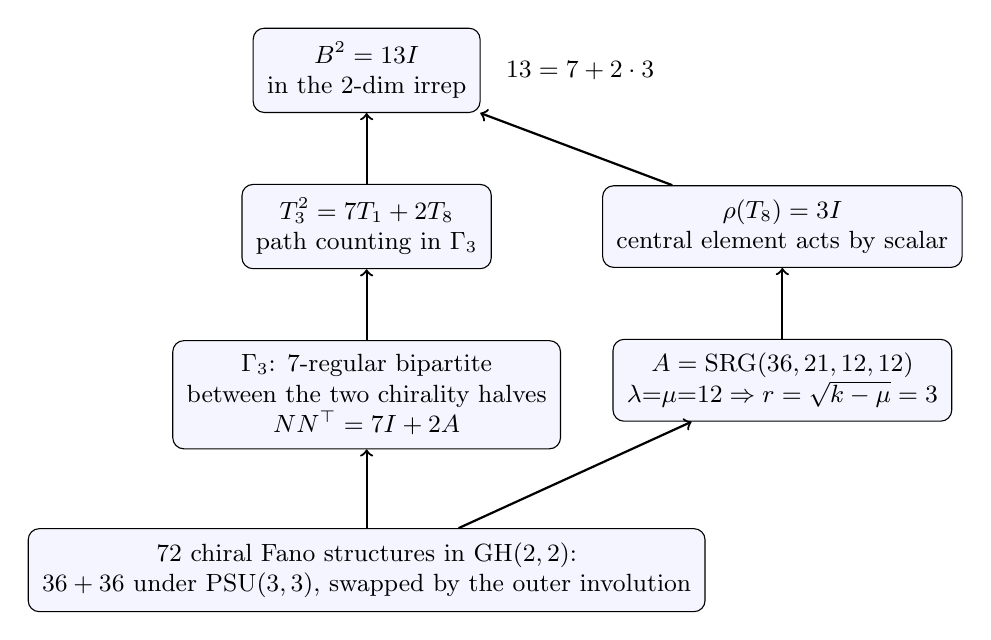
\begin{tikzpicture}[
  box/.style={draw, rounded corners, align=center, font=\small,
              inner sep=5pt, fill=blue!4},
  arr/.style={->, thick},
  node distance=9mm and 6mm]
\node[box] (b2)   {$B^2 = 13I$ \\ in the $2$-dim irrep};
\node[box, below=of b2] (t3)  {$T_3^2 = 7T_1 + 2T_8$ \\ path counting in $\Gamma_3$};
\node[box, right=14mm of t3] (t8)  {$\rho(T_8) = 3I$ \\ central element acts by scalar};
\node[box, below=of t3] (bip) {$\Gamma_3$: $7$-regular bipartite \\ between the two chirality halves \\ $NN^\top = 7I + 2A$};
\node[box, below=of t8] (srg) {$A = \mathrm{SRG}(36,21,12,12)$ \\ $\lambda{=}\mu{=}12 \Rightarrow r = \sqrt{k-\mu} = 3$};
\node[box, below=10mm of bip] (geo) {$72$ chiral Fano structures in $\GH(2,2)$:\\
$36 + 36$ under $\PSU(3,3)$, swapped by the outer involution};
\draw[arr] (t3) -- (b2);
\draw[arr] (t8) -- (b2);
\draw[arr] (bip) -- (t3);
\draw[arr] (srg) -- (t8);
\draw[arr] (geo) -- (bip);
\draw[arr] (geo) -- (srg);
\node[right=2mm of b2, font=\small] {$13 = 7 + 2\cdot 3$};
\end{tikzpicture}
\caption{The logical chain behind $B^2 = 13I$.}
\label{fig:chain}
\end{figure}

%======================================================================
\section{Connections}\label{sec:connections}
%======================================================================

\begin{enumerate}
\item \textbf{Fano $\leftrightarrow$ hexagon, structurally.} Both are thick
generalized polygons of order $(2,2)$: $n = 3$ and $n = 6$ in the
Feit--Higman list. The Fano plane's incidence graph is the Heawood graph
(girth $6$); the hexagon's incidence graph has girth $12$. The hexagon is,
in a precise sense, the ``girth-doubled'' sibling --- and by
Theorem~\ref{thm:subhexagon} this is not just an analogy: the
girth-doubling of the Fano plane (its flag geometry, a thin hexagon of
order $(2,1)$, incidence graph $=$ subdivided Heawood graph) literally
embeds in $\mathrm H(2)$, in exactly $36$ ways.
\item \textbf{Fano $\leftrightarrow$ hexagon, via octonions.} Fano $=$
multiplication chart of compact octonions
(Definition~\ref{def:fano-oct}); hexagon $=$ null geometry of split
octonions (Definition~\ref{def:hex-octonion}). Same exceptional algebra,
two forms.
\item \textbf{Fano $\leftrightarrow$ hexagon, via subgroups.}
$\Aut(\text{Fano}) = \PSL(3,2)$ of order $168$ embeds in
$\Aut(\mathrm H(2)) = G_2(2)$ of order $12096$ with index $72$; each
embedded copy paints a chiral Fano structure (two spreads on a
$21$-point orbit) onto the hexagon, and the $21$-orbit is the flag set of
that Fano plane: $21 = $ flags, $42 = $ antiflags
(Fact~\ref{fact:fano-aut} meets Proposition~\ref{prop:orbits}).
\item \textbf{The number 14, three ways.} $\deg\chi_{14} = 14$ is:
the multiplicity of eigenvalue $-3$ in the $63$-point collinearity graph;
the multiplicity of $\pm\sqrt{13}$ in $\Gamma_3$; the multiplicity of the
$2$-dim irrep in $\C[G/K]$. Also $14 = \dim G_2$ (the Lie algebra!) ---
$\chi_{14}$ is the ``adjoint-flavoured'' irreducible of $G_2(2)$.
\item \textbf{The number 13 elsewhere?} $13 = |\,\mathrm{points\ of\ }
\PG(2,3)|$ is surely coincidence; but $13 = 14 - 1$ and the
$\chi_{14}$-isotypic block carrying eigenvalue $13$ has dimension
$28 = 2\cdot 14$ --- see Open Questions.
\item \textbf{Same theorem, two costumes.} ``$B^2 = 13I$'' and ``the
bipartite halved graph of $\Gamma_3$ has $NN^\top = 7I + 2A_{\rm SRG}$''
are the \emph{same} statement, once in Wedderburn coordinates, once in
adjacency coordinates. Likewise $AB + BA = -4I$ is the $U_3(3)$-graph
eigenvalue $-4$ in Wedderburn coordinates
(Corollary~\ref{cor:restatements}).
\end{enumerate}

%======================================================================
\section{Open questions}\label{sec:open}
%======================================================================

\begin{question}[Synthetic proof of $T_3^2 = 7T_1 + 2T_8$]
Find a purely geometric proof, in the language of spreads in $\GH(2,2)$,
that two chiral Fano structures in relation $D_8$ are connected by exactly
$2$ structures in relation $D_3$ to both, while structures in relations
$D_4, D_6, D_7$ are connected by none. A positive answer would replace the
GAP certificate in Proposition~\ref{prop:pathcount} and likely explain the
coefficient $2$ as ``the two points of a hexagon line off a given point''
or similar. A negative-style outcome (no clean synthetic argument) would
suggest the right level of abstraction is the association scheme, not the
geometry.
\end{question}

\begin{question}[Why $\lambda = \mu$?]
The clean form $13 = 7 + 2\sqrt{k-\mu}$ relies on
$\mathrm{SRG}(36,21,12,12)$ having $\lambda = \mu = 12$, i.e.\ being a
\emph{conference-like} graph in the $(\lambda{=}\mu)$ family
($k = \lambda + \sqrt{k-\mu}\,$?). Is there a geometric reason the
$36$ Fano structures of one chirality form an SRG with $\lambda = \mu$?
(E.g.\ a $2$-design structure on the $36$.) Partial progress: $\lambda =
\mu$ holds iff the SRG eigenvalues are $\pm\sqrt{k-\mu}$, iff the
two-dimensional Hecke block has $\mathrm{tr}\,\rho(T_8') = 0$ for the
relevant element --- an algebra-level reformulation, not yet an
explanation.
\end{question}

\begin{question}[$13 = 14 - 1$?]
Is there natural meaning to $13 = \deg\chi_{14} - 1$, e.g.\ via the action
on the $14$-dimensional module with a fixed vector removed? A positive
answer would connect $B^2 = 13I$ to the Lie-theoretic $14 = \dim G_2$. A
counterexample shape: an analogous Hecke algebra (next $q$?) where the
matching numerology fails.
\end{question}

\begin{question}[$q$-analogue]
For $G_2(q) \supset \PSL(3,q)$ (when the embedding exists, $q = p \geq 2$):
does the double-coset algebra have rank $8$, and is there a polynomial
$13(q)$ with $13(2) = 13$? Guess shapes: $q^3 + q + \ldots$, or
$7 + 2\cdot 3 \to (q^2{+}q{+}1) + 2\cdot$? Computing $q = 3$
($G_2(3)$, index of $\PSL(3,3) = $ ?) is the obvious experiment; it may be
too large for naive GAP double-coset enumeration but the orbital method of
\texttt{why13\_orbitals.g} scales.
\end{question}

\begin{question}[$|P \cap P'| = 9$ coincidence?]
For $\Gamma_3$-adjacent structures, $|P\cap P'| = 9 = k - \mu$. Same number
as in $\sqrt{k-\mu} = 3$. Coincidence or mechanism?
\end{question}

%======================================================================
\section*{Sources}
%======================================================================
\begin{itemize}
\item J. Tits, \emph{Sur la trialit\'e et certains groupes qui s'en
d\'eduisent}, Publ.\ Math.\ IH\'ES 2 (1959), 13--60. [Hexagon
construction, Definition~\ref{def:hex-quadric}.]
\item W. Feit, G. Higman, \emph{The nonexistence of certain generalized
polygons}, J.\ Algebra 1 (1964), 114--131. [Fact~\ref{fact:feithigman}.]
\item A. M. Cohen, J. Tits, \emph{On generalized hexagons and a near
octagon whose lines have three points}, European J.\ Combin.\ 6 (1985),
13--27. [Fact~\ref{fact:cohentits}.]
\item H. Van Maldeghem, \emph{Generalized Polygons}, Monographs in
Mathematics 93, Birkh\"auser 1998. [General reference; coordinates for
Definition~\ref{def:hex-quadric}.]
\item Conway et al., \emph{ATLAS of Finite Groups}. [$G_2(2) = U_3(3){:}2$,
the $U_3(3)$ graph, character degrees $1,1,6,7,14,21,27,\dots$]
\item D. R. Hughes, F. C. Piper, \emph{Projective Planes}, Springer 1973.
[Theorem~\ref{thm:fano-unique} and plane axiomatics.]
\item P. J. Cameron, J. H. van Lint, \emph{Designs, Graphs, Codes and their
Links}, CUP 1991. [SRG eigenvalue formulas, Proposition~\ref{prop:srg}.]
\item A. De Wispelaere, H. Van Maldeghem, \emph{Codes from generalized
hexagons}, Des.\ Codes Cryptogr.\ 37 (2005), 435--448. [The $36$
distance-$2$ ovoids of $\mathrm H(2)$, Fact~\ref{fact:priorart}(1).]
\item B. De Bruyn, P. Vandecasteele, \emph{A characterization of the split
Cayley generalized hexagon $H(q)$ using one subhexagon of order $(1,q)$},
Discrete Math.\ 294 (2005). [Theorem~\ref{thm:subhexagon} context.]
\item R. Gramlich, M. Horn, A. Pasini, H. Van Maldeghem, \emph{Intransitive
geometries and fused amalgams}, J.\ Group Theory 11 (2008),
arXiv:0708.3515. [$\PSL(2,7)$-substructures of $G_2$-geometries.]
\item P. L\'evay, M. Saniga, P. Vrana, arXiv:0808.3849 (2008). [Fano
subplanes and Heawood subgraphs of $\mathrm H(2)$ in three-qubit physics.]
\item A. E. Brouwer, graph descriptions at
\texttt{aeb.win.tue.nl/graphs/U3\_3.html} and
\texttt{.../Heawood.html}; A. E. Brouwer, H. Van Maldeghem,
\emph{Strongly Regular Graphs}, CUP 2022. [Fact~\ref{fact:priorart}(3).]
\item A. Inoue, \emph{An alternative construction of the $G_2(2)$-hexagon},
arXiv:2501.04725 (2025); \emph{An alternative construction of the
$G_2(2)$-graph}, arXiv:2601.12235 (2026). [Recent closely related work.]
\item A. Hanaki, I. Miyamoto, association scheme database,
\texttt{math.shinshu-u.ac.jp/\textasciitilde hanaki/as/}. [Classification
stops below $72$ vertices; Fact~\ref{fact:priorart}(4).]
\item This repository: \texttt{MEINHOLD-HECKE.md} (multiplication table,
Wedderburn data), \texttt{why13\_fano.g}, \texttt{why13\_orbitals.g},
\texttt{why13\_subhexagon.g}, \texttt{why13\_classes.g},
\texttt{why13\_orbitals.out} (all computations).
\end{itemize}

\end{document}
